\documentclass{article}
\usepackage[english]{babel} % Changed to English
\usepackage[T1]{fontenc}
\usepackage{graphicx}   % For including images
\usepackage{fancyhdr}   % For customizing headers and footers
\usepackage{tabularx}
\usepackage{subcaption} % For subcaptions in figures
\usepackage{placeins}   % For \FloatBarrier to control float placement
\usepackage{float}
\usepackage{wrapfig}    % For wrapfigure environment
\usepackage{tikz}       % For drawing diagrams
\usetikzlibrary{decorations.pathreplacing} % For brace decoration in TikZ
\usetikzlibrary{angles, quotes, positioning, arrows.meta}   
\usetikzlibrary{calc} % For coordinate calculations in TikZ
\usepackage{amsmath}    % For \text and other math features
\usepackage{booktabs}   % For \toprule, \midrule, \bottomrule in tables
% \usepackage{bibentry}
% \nobibliography*
\usepackage{url}
\usepackage[hidelinks]{hyperref}
\hypersetup{urlcolor=blue}
\usepackage[numbers]{natbib}
\usepackage{doi}
\usepackage{titlesec} % Added for \titleformat command

% Suppress subfigure labels (a), (b), etc.
\captionsetup[subfigure]{labelformat=empty}

% Set up the header and footer
\fancyfoot[R]{
\includegraphics[height=.75cm]{imgs/unilr_logo.png}} % Logo on the right
\fancyfoot[L]{NGUYEN Hoang Nhat}                             % Name on the left
\fancyfoot[C]{\thepage}                              % Page number centered
\renewcommand{\footrulewidth}{0.5pt}                 % Line above footer
\renewcommand{\headrulewidth}{0pt}                   % Remove the header line
\fancyhead{}                                         % Clear all header content
\pagestyle{fancy}                                    % Apply fancy style to all pages after title

% Beginning the document
\begin{document}
\pagenumbering{gobble} % Suppress page numbering on the title page

% Centering all content for the cover page
\begin{center}

% Including logos side by side
\begin{minipage}{0.7\textwidth}
    
\includegraphics[height=3cm]{imgs/mia_logo.png}
    \hfill
\end{minipage}
\hfill
\begin{minipage}{0.29\textwidth}
    \hfill
    
\includegraphics[height=3cm]{imgs/unilr_logo.png}
\end{minipage}
\vspace{1cm}

% Adding horizontal lines above and below the title section
\noindent\rule{\textwidth}{2pt}

% Adding the title of the report
{\Huge \textbf{Internship Report}\par}
\vspace{1cm}

% Adding the specific topic of the internship
{\Large \textbf{Detection and Semantic Segmentation on Meta Quest 3}\par}

\noindent\rule{\textwidth}{2pt}

\vspace{1cm}

% Adding the author's name
{\Huge \textbf{NGUYEN Hoang Nhat}\par}
\vspace{1cm}

% Adding the internship period
{\large \textbf{Internship Period: April 20, 2026 -- June 19, 2026}\par}
\vspace{1cm}

% Adding the institution and laboratory details
{\large \textbf{Laboratoire Mathématiques, Image et Applications}\par}
{\large \textbf{La Rochelle Université}\par}
\vspace{1.5cm}

% Overview image
% \begin{figure}[H]
%     \centering
%     \includegraphics[height=3cm]{imgs/project_title_image.png}
% \end{figure}

% Adding submission date and tutor/supervisor details side by side
\begin{minipage}{0.49\textwidth}
    \raggedright
    {\large \textbf{Submitted on:}\\ 29/5/2026\par}
\end{minipage}
\begin{minipage}{0.49\textwidth}
    \raggedleft
    {\large \textbf{Supervisor:}\\ Péteri Renaud }\\
    {\large \textbf{University tutor:}\\ Mascarilla Laurent  }
\end{minipage}

\end{center}

% Ensuring no page number appears
\thispagestyle{empty}

\newpage
\vspace*{2cm}
\begin{center}
    {\LARGE Acknowledgements}
\end{center}
\vspace{1cm}
    
I would like to express my greatest gratitude to my supervisor, Mr.Péteri, for his warm welcome and thorough support during my internship at the MIA laboratory. His availability and thoughtful guidance provided me with a wonderful experience and a significant contribution to my personal growth.\\

My thanks also go to my university tutor, Mr. Mascarilla, for his oversight and support throughout this period. Last but not least, I want to convey my deep gratitude to the La Rochelle Université and the MIA laboratory for allowing me to have this valuable opportunity, which profoundly enhanced my skills and knowledge during my Bachelor of Computer Science.\\

This experience has been vastly rewarding and has further strengthened my professional career. Thank you all for making this opportunity available. 


\newpage
\tableofcontents

\newpage
\section{Introduction} % add more context, capture device etc.
\pagenumbering{arabic} % Start page numbering from 1
\setcounter{page}{1}

\subsection{Internship Overview}
This report presents my work, which was based on the I-WRIST project (ANR), conducted during my internship at the \textit{Laboratoire Mathématiques Image Applications} (MIA), commencing on April 20, 2026. \\

% (MIA lab overview)\\
The MIA Laboratory, established in 2008, specializes in applied mathematics, image processing, and computer science, and is a member of the LUDI Institute (Littoral Urbain Durable Intelligent) at La Rochelle Université, as well as the FREDD, MIRES, and MARGAUX research federations. Directed by Catherine Choquet, MIA comprises a multidisciplinary team of 22 researchers, with expertise in signal processing, computer vision, and machine learning.\\

% (My project overview)\\
My internship's goal is to experiment the possibilities of running computer vision algorithms on the Meta Quest 3 device in an Augmented Reality setting. \\


My work focused on developing a gaze-based object detection and segmentation on the Meta Quest 3 device to enhance the functionality of upper limb prostheses. My internship was conducted on-site at the MIA Laboratory in La Rochelle, primarily under the supervision of Mr. Péteri.


\subsection{The IWRIST Project}

The primary objective of IWRIST Project (ANR) - Intuitive Wrist Prosthesis Control Based on natural movement and visual information (2024-2028) - is to empower individuals with above-elbow amputations to control robotic prosthetic arms using gaze data. Traditional myoelectric control systems, which rely on residual muscle signals, often fall short in managing the multiple degrees of freedom required for complex tasks. To address this limitation, computer vision techniques, leveraging gaze data captured by wearable devices, provide a promising solution for identifying and tracking objects of interest for grasping tasks. This approach aims to improve the precision and intuitiveness of prosthetic control, thereby enhancing the quality of life for amputees.\\


% (Members, multidisciplinary)\\
The IWRIST a joint project between Université de Bordeaux, Université de La Rochelle, Pollen Robotics and La Tour de Gassie. The members consists of a disciplinary team of computer vision scientists, biomechanics, robotics engineers, cognitive scientists, and physicians. \\

% (Issues regarding the hololens 2 -> in need of other devices like Meta Quest 3 as well as on-device inference)\\
So far, one of the challenges of the IWRIST project is that the device they have been using, the Hololens 2, has been scheduled for discontinuity. This called for the use of alternative devices, one of which was the Meta Quest 3, developed by Meta. Additionally, the processing of project's pipeline has been mostly done on a separate GPU (RTX 40s series) and the possibility of on-device inference is being taken into consideration.\\

The Meta Quest 3 device has recently allowed developers to access raw pixel data in 2025, and since then, it has been considered as a suitable tool for computer vision tasks. The device itself is significantly more affordable, with only a sixth of the cost of the Hololens 2. It provides a similar processing power, receives active updates, and inherits access to an abundance of tools from Meta's ecosystem. However, the device still presents some limitations, for example, the lack of a built-in eye tracking tool.

\subsection{My Project}
\subsubsection{Project Context and Objectives}

This project's goal is to evaluate the feasibility of deploying on-device AI inference by developing a simplified pipeline of the IWRIST project's. Because the Meta Quest 3 lacks integrated eye-tracking hardware, this work utilizes \textbf{head-gaze (the directional vector of the headset)} as a baseline proxy for visual attention. The results can then be later utilized by IWRIST's team for possible development on the Meta Quest 3. This project also took an attempt to optimize dataflow to enhance performance on the edge-device.\\

Below is how my project fits into the IWRIST's pipeline

\begin{figure}[htbp]
\centering
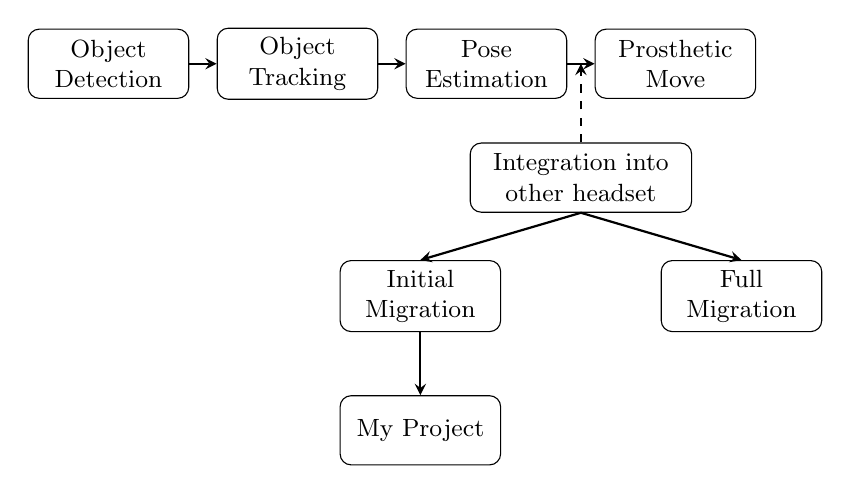
\begin{tikzpicture}[
    % Tighter spacing between non-absolute nodes
    node distance=0.8cm and 0.3cm, 
    box/.style={rectangle, draw, rounded corners, minimum height=2.5em, minimum width=5.8em, align=center, font=\small},
    arrow/.style={-stealth, thick},
    dashed arrow/.style={-stealth, thick, dashed}
]
    % 1. Core Horizontal Pipeline (Brought closer together: 0 -> 2.4 -> 4.8 -> 7.2)
    \node[box] (b1) at (0,0) {Object\\ Detection};
    \node[box] (b2) at (2.4,0) {Object\\ Tracking};
    \node[box] (b3) at (4.8,0) {Pose\\ Estimation};
    \node[box] (b4) at (7.2,0) {Prosthetic\\ Move};

    % 2. Core Pipeline Arrows & Midpoint Coordinate
    \draw[arrow] (b1) -- (b2);
    \draw[arrow] (b2) -- (b3);
    \draw[arrow] (b3) -- (b4) coordinate[midway] (mid);

    % 3. New Nodes (Stacked tighter vertically and horizontally)
    \node[box] (integration) [below=1.0cm of mid, minimum width=8em] {Integration into\\ other headset};
    
    \node[box] (initial) [below left=0.6cm and -0.4cm of integration] {Initial\\ Migration};
    \node[box] (full) [below right=0.6cm and -0.4cm of integration] {Full\\ Migration};
    
    \node[box] (myproject) [below=of initial] {My Project};

    % 4. Connecting New Arrows
    \draw[dashed arrow] (integration.north) -- (mid);
    \draw[arrow] (integration.south) -- (initial.north);
    \draw[arrow] (integration.south) -- (full.north);
    \draw[arrow] (initial.south) -- (myproject.north);

\end{tikzpicture}
\caption{The four-step IWRIST pipeline and the possible migration to the Meta Quest 3, which includes my work.}
\label{fig:headset-integration-flow}
\end{figure}

\subsubsection{Timeline}

A approximate overview of the different phases of my internship is provided bellow in Figure~\ref{fig:gantt}, with the red line indicating the date when this report was writen.


\begin{figure}[H]
    \centering
    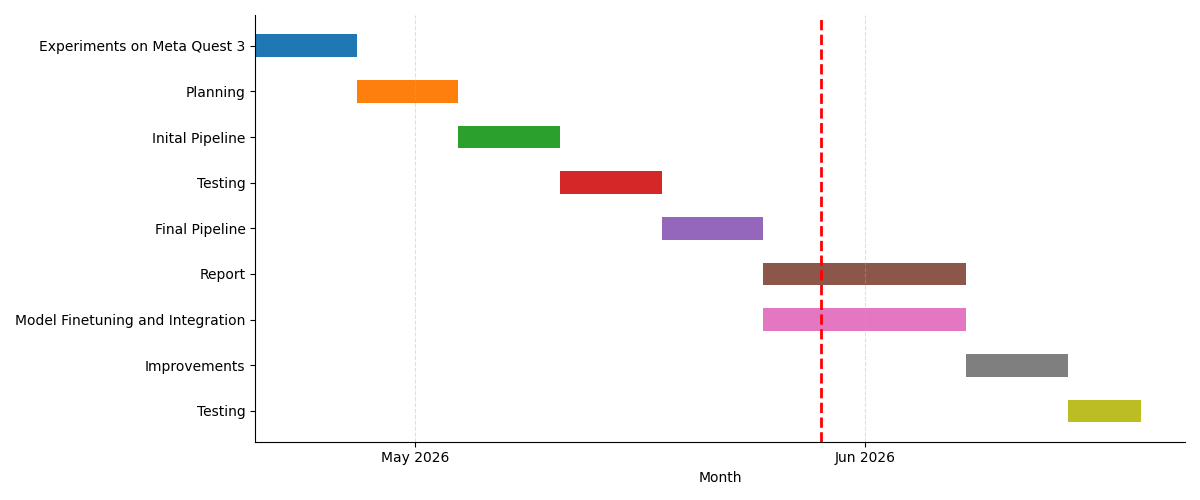
\includegraphics[width=\linewidth]{imgs/gannt_chart.png}
    \caption{Chart showing the approximate timeline and phases of the internship project}
    \label{fig:gantt}
\end{figure}
% Phase, start date, duration
% data = [
%     ["Experiments on Meta Quest 3", "2026-04-20", 7],
%     ["Planning", "2026-04-27", 7],
%     ["Inital Pipeline", "2026-05-04", 7],
%     ["Testing", "2026-05-11", 7],
%     ["Final Pipeline", "2026-05-18", 7],
%     ["Report", "2026-05-25", 14],
%     ["Model Finetuning and Integration", "2026-05-25", 14],
%     ["Improvements", "2026-06-08", 7],
%     ["Testing", "2026-06-15", 5],
% ]

I took the first week to familiarize myself with the headset and its utilities. Then another week was used to plan the timeline and to come up with ideas for the pipeline, about which I discussed with my supervisor. The rest of the phases mostly matched the plan, except for the model integration which is taking longer than expected.

\subsubsection{Pipeline}
The system is structured around four key phases: object detection, head gaze selection, region of interest (ROI) cropping, and semantic segmentation. 
\begin{figure}[H]
\centering
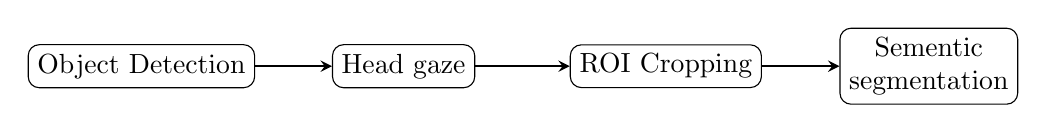
\begin{tikzpicture}[
    box/.style={rectangle, draw, rounded corners, align=center},
    arrow/.style={-stealth, thick}
]
    \node[box] (b1) at (0,0) {Object Detection};
    \node[box] (b2) at (3.33,0) {Head gaze};
    \node[box] (b3) at (6.66,0) {ROI Cropping};
    \node[box] (b4) at (10,0) {Sementic \\segmentation};
    \draw[arrow] (b1) -- (b2);
    \draw[arrow] (b2) -- (b3);
    \draw[arrow] (b3) -- (b4);
\end{tikzpicture}
\caption{Overview of the pipeline.}
\label{fig:pipeline-overview}
\end{figure}

The pipeline, illustrated in Figure~\ref{fig:pipeline-overview}, consists of the following stages:

\begin{itemize}
    \item \textbf{Object Detection}: This stage uses a light-weight multi-detection on the camera frame and use depth to display the bounding boxes on the real world (Augmented Reality).
    
    \item \textbf{Head Gaze Object Selection}: After the bounding boxes have appeared, the direction of the headset is used to point to the bounding box, which selects it and displays the json description of the object.
    
    \item \textbf{ROI Cropping}: The selected bounding box (+10\% around the box) is used as a region of interest, which is then passed to the segmentation phase
    
    \item \textbf{Semantic Segmentation}: Finally the selected ROI is passed to a light-weight semantic segmentation model and a mask is displayed on the real world (Augmented Reality).
\end{itemize}

To support the development and evaluation of the project, a diverse dataset were employed. The following sections detail this dataset, along with the performance metrics used to assess the system's effectiveness.

% \newpage
\section{Datasets Used}

In this project, we utilize the "Grasping in the Wild" dataset \cite{graspinginthewild}, available on \href{https://universe.roboflow.com/iwrist/grasping-in-the-wild}{\textbf{RoboFlow}}. The semantic segmentation annotations for this corpus were developed under the framework of the I-Wrist Project \cite{atoki2024object}. This dataset provides diverse scenarios for developing and evaluating the entire pipeline.\\

The \textbf{Grasping In The Wild} (GITW) dataset is a comprehensive collection of egocentric video sequences capturing everyday objects, such as plates, bowls, and frying pans, in naturalistic, cluttered environments like kitchens. This dataset poses significant challenges for object tracking due to its complex backgrounds and varying lighting conditions, making it an ideal testbed for real-world applications.

\begin{figure}[H]
    \centering
        \begin{subfigure}[b]{0.32\textwidth}
            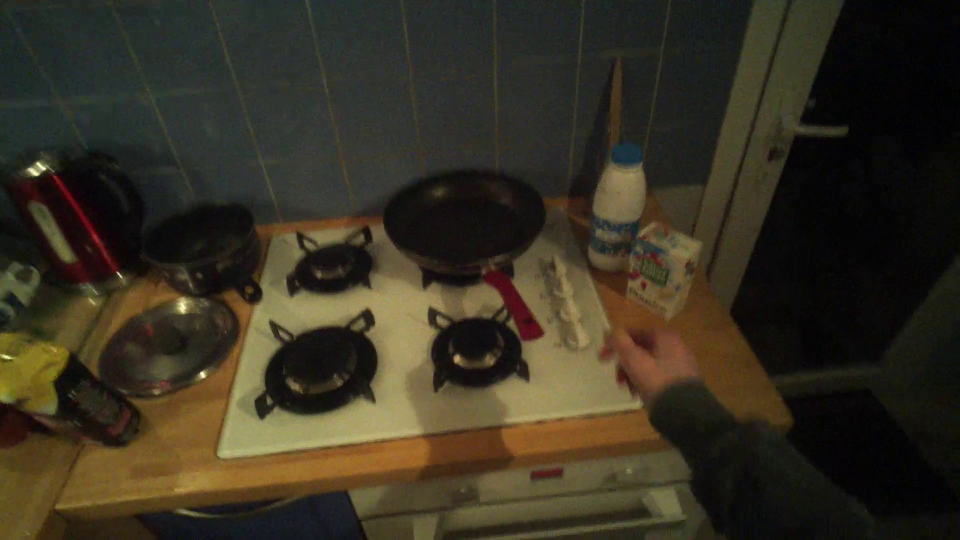
\includegraphics[width=\linewidth]{imgs/dataset_sample_pan.png}
            \caption{Frying pan example}
        \end{subfigure}
        \hfill
        \begin{subfigure}[b]{0.32\textwidth}
            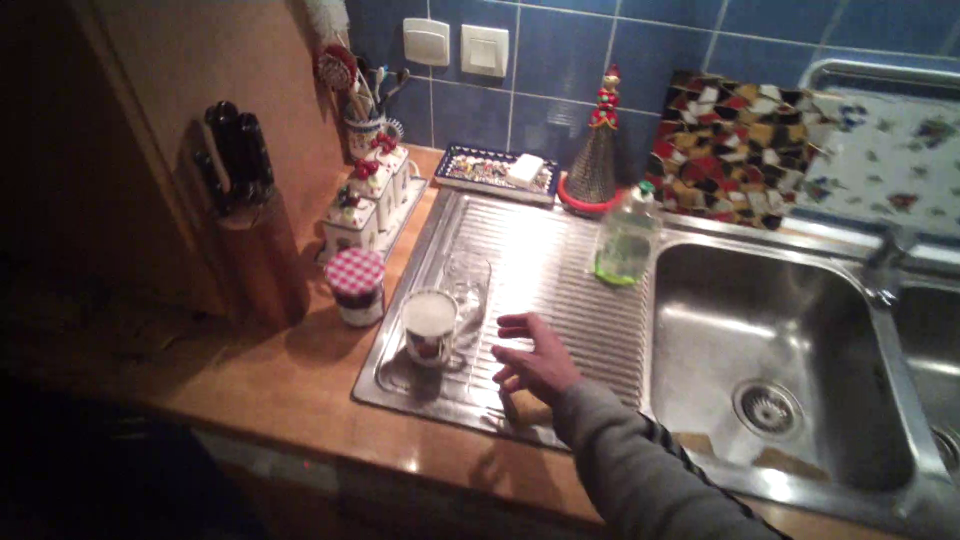
\includegraphics[width=\linewidth]{imgs/dataset_sample_mug.png}
            \caption{Mug example}
        \end{subfigure}
        \hfill
        \begin{subfigure}[b]{0.32\textwidth}
            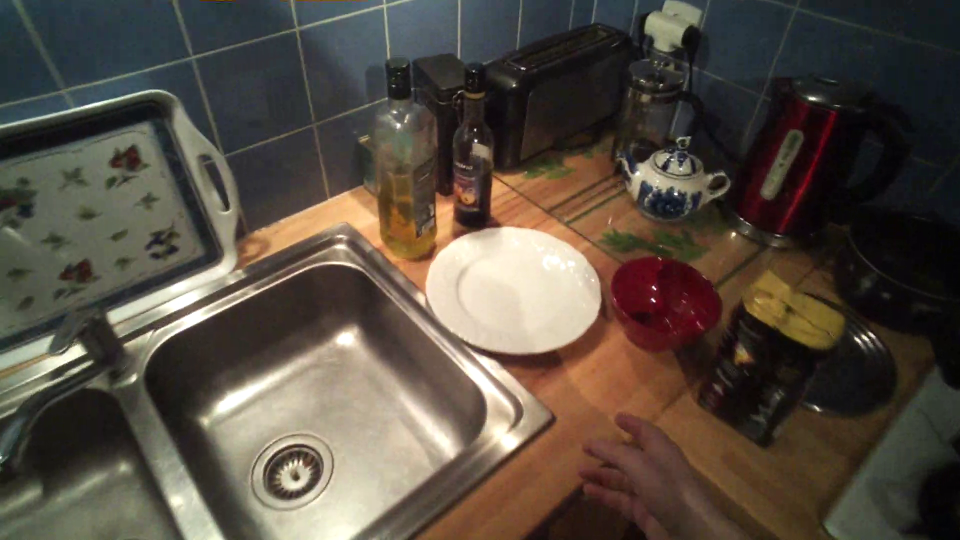
\includegraphics[width=\linewidth]{imgs/dataset_sample_plate.png}
            \caption{Plate example}
        \end{subfigure}
        \caption{Sample frames from the GITW dataset.}
        \label{fig:gitw-sample-frames}
\end{figure}

The data was recorded using the \textit{Tobii Pro Glasses 2}, a wearable eye-tracking device that captures RGB video at 25 Hz and gaze fixation points at 50 Hz. The dataset includes manually annotated binary masks for the objects of interest in each frame, providing ground truth segmentations that facilitate the benchmarking of the semantic segmentation. With 16 object classes and over 13,000 annotated frames, the GITW dataset allows for robust evaluation in diverse, real-world scenarios.


\newpage
\section{Metrics and Evaluation}

This section outlines the evaluation metrics used to assess the performance of the detection and segmentation system, focusing on the object tracking and 3D object shape extraction phases of the pipeline. The primary metrics employed are Intersection over Union (IoU) and Mean Average Precision , which provide robust measures of detection and segmentation accuracy across the Grasping In The Wild (GITW) dataset.

\subsection{Intersection over Union (IoU)}

Intersection over Union (IoU) \cite{IoU}, also known as the Jaccard Index, is a widely adopted metric used in both object detection and semantic segmentation to measure how well predicted regions match ground truth. It measures the overlap between a prediction (\(M\)) and the ground truth (\(\bar{M}\)) for a given video frame \(f\), as defined by the following equation:

$$\text{IoU}_f = \frac{|M \cap \bar{M}|}{|M \cup \bar{M}|}$$

For object detection, \(|M \cap \bar{M}|\) represents the number of pixels in the intersection of the predicted and ground truth \textbf{box}, and \(|M \cup \bar{M}|\) denotes the number of pixels in their union. \\

For semantic segmentation, \(|M \cap \bar{M}|\) represents the number of pixels in the intersection of the predicted and ground truth \textbf{masks}, and \(|M \cup \bar{M}|\) denotes the number of pixels in their union. \\

The IoU score ranges from 0 to 1, with a value of 1 indicating perfect overlap and 0 indicating no overlap.

% For a video sequence of \(N\) frames, the mean IoU (mIoU) is computed as the average IoU across all frames:

% $$\text{mIoU} = \frac{1}{N} \sum_{i=1}^N \text{IoU}_{f_i}$$

% In the context of this project, IoU is used to evaluate the accuracy of the object masks generated during the segmentation phase. For the GITW dataset, which contains manually annotated ground truth masks for 16 object classes in cluttered environments, IoU provides a precise measure of how well the system tracks objects under challenging conditions. 

\subsection{Average Precision (AP)}

Average Precision (AP) \cite{mAP} is a widely used evaluation metric in object detection that measures both the classification and localization performance of a model. It summarizes the trade-off between precision and recall across different confidence thresholds using the area under the Precision--Recall (PR) curve.\\

For a given class \(c\), precision and recall are defined as:

$$
\text{Precision}_c = \frac{TP_c}{TP_c + FP_c} 
\qquad \text{and} \qquad 
\text{Recall}_c = \frac{TP_c}{TP_c + FN_c}
$$

where \(TP_c\), \(FP_c\), and \(FN_c\) denote the number of true positives, false positives, and false negatives for class \(c\), respectively. A predicted detection is considered a true positive only if:
\begin{itemize}
    \item the predicted class matches the ground truth class, and
    \item the Intersection over Union (IoU) exceeds a predefined threshold.
\end{itemize}

By varying the confidence threshold of the detector, a Precision--Recall curve is generated. For discrete evaluations across $N$ threshold levels, the Average Precision is approximated as:

$$ AP_c = \sum_{k=1}^{N} P_c(k) \Delta R_c(k) $$

where $P_c(k)$ is the precision at the $k$-th threshold, and $\Delta R_c(k)$ represents the change in recall between thresholds $k$ and $k-1$.

\newpage
\section{The Meta Quest 3 device}
The \href{https://www.meta.com/quest/quest-3/}{Meta Quest 3} is a standalone virtual and mixed reality headset powered by Meta Horizon OS. It features major architectural upgrades over the Quest 2, including a 40\% thinner enclosure achieved through pancake optics, dedicated hardware for full-color stereoscopic passthrough, and a built-in depth sensor for environment mapping.

\begin{figure}[H]
    \centering
    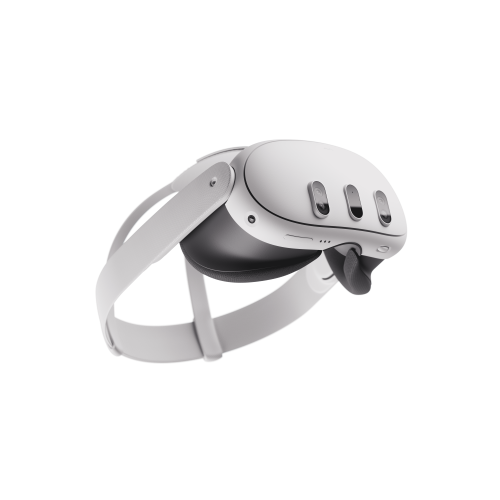
\includegraphics[width=0.35\linewidth]{imgs/mq3.png}
    \label{fig:placeholder}
\end{figure}

Below is the specifications of the device :

\begin{table}[H]
\centering
\label{tab:quest3_specs}
% \textwidth forces the table to fit the page; X dynamically sizes and wraps the column
\begin{tabularx}{\textwidth}{p{3.8cm} X}
\hline
\textbf{Component / Feature} & \textbf{Specification Detail} \\ \hline
\textbf{Processor (SoC)}     & Qualcomm Snapdragon XR2 Gen 2 (Adreno 740 GPU) \\ 
\textbf{Memory}              & 8~GB LPDDR5 RAM \\ 
\textbf{Display Resolution}  & Dual LCD panels, $2064 \times 2208$ pixels per eye \\ 
\textbf{Optics}              & $2\times$ element custom pancake lenses \\ 
\textbf{Refresh Rate}        & 90~Hz – 120~Hz \\ 
\textbf{IPD Adjustment}      & Mechanical scroll wheel (Continuous range: $53\text{~mm} - 75\text{~mm}$) \\ 
\textbf{Cameras \& Sensors}  & $2\times$ 4~MP RGB color cameras (Passthrough), $4\times$ $400 \times 400$ px IR tracking cameras, $1\times$ IR depth sensor \\ 
\textbf{Controllers}         & Ringless ``Touch Plus'' controllers with haptic feedback \\ 
\textbf{Weight}              & 515 grams \\ \hline
\textbf{Current Cost (2026)}  & \$599.99 (512~GB)\\ \hline
\end{tabularx}
\caption{Meta Quest 3 Specifications}
\end{table}

\newpage
\section{Utilities}

This section shows the important utilities used in this project.
This project's initial implementation was built from the workflow provided in the official Meta Quest Passthrough API sample codebase \cite{oculus_passthrough_samples}.

\subsection{Meta Extended Reality SDK}

The Meta Extended Reality (XR) SDK provides a collection of tools and APIs for developing immersive applications on Meta Quest devices. It enables developers to integrate virtual reality (VR), augmented reality (AR), and Augmented reality (MR) functionalities, including spatial understanding, passthrough rendering, and environment interaction.

\subsubsection{Passthrough Camera Access}

Recent updates to the Meta XR SDK introduced support for accessing raw \href{https://developers.meta.com/horizon/documentation/spatial-sdk/spatial-sdk-pca-overview/}{\textbf{Passthrough camera}} data on Meta Quest devices. Since 2025, developers are able to retrieve pixel-level image data directly from the headset cameras, enabling advanced computer vision applications.\\

This capability allows applications to perform tasks such as: object detection, semantic segmentation, marker tracking, scene understanding, and real-time AI-assisted interactions.

\subsubsection{Environment Raycast}

The \href{https://developers.meta.com/horizon/documentation/unity/unity-mr-utility-kit-environment-raycast/}{\textbf{Environment Raycast system}} provides spatial querying capabilities that allow virtual content to interact accurately with the real-world environment. Raycasting uses spatial mapping and depth estimation to determine intersections between virtual rays and detected physical surfaces.\\

This functionality allows a more accurate placement of the bounding boxes and segmentation masks obtained in this pipeline.

\subsection{Unity Game Engine}
% (Overview)\\
\textbf{Unity} is a cross-platform real-time development engine widely used for developing video games and extended reality (XR) applications. It provides an integrated environment for rendering, physics simulation, user interaction, and deployment across multiple platforms, including Meta Quest headsets. So far, this has been the main way of developing applications on Meta Quest 3.

% (so far the main way of app development on Meta Quest)\\

\subsubsection{Sentis (Inference Engine) framework}

% (Overview)\\
\href{https://docs.unity3d.com/Packages/com.unity.ai.inference@2.2/manual/index.html}{\textbf{Unity Sentis}} is Unity's neural network inference framework designed for running machine learning models directly inside applications made by the Unity engine. \\

% (Limitations, compared to OpenCV)\\
However, compared to \textbf{OpenCV}, Sentis offers less low-level computer vision utilities and instead focus on integration for deploying deep learning models in applications.


% \newpage
\section{Object Detection}
\label{sec:detection}

\subsection{Overview}
Object detection is the first stage of the pipeline. Every other frame captured by the
passthrough camera is fed to a detection model that returns bounding boxes
and class labels for all objects of interest visible in the scene. These boxes are then
rendered as overlays and exposed to the head-gaze selector, which uses
them as entry points for the segmentation stage.
% ─────────────────────────────────────────────────────────────────────────────
\subsection{Model Choice}
\label{sec:det-model-choice}

The primary constraint governing model selection is real-time performance on the
Meta Quest~3. The pipeline runs asynchronously on the Snapdragon XR2 Gen~2 GPU via Unity Sentis'
Vulkan compute backend. A secondary constraint is model file size, since the model
must be bundled with the application and quantised for storage.

\paragraph{YOLOv8n.}
\texttt{YOLOv8n}~ is the nano variant of Ultralytics' YOLOv8 family,
released in January 2023. It achieves a mAP\textsuperscript{box}$_{50\text{--}95}$ of 37.3 on the COCO val2017 benchmark~at 3.2\,M parameters and
approximately 6\,MB on disk (FP32 ONNX). It has been the industry standard for several computer vision tasks on edge-device. Several properties make it well-suited to this application:

\begin{itemize}
    \item \textbf{ONNX export and Sentis compatibility.} The model exports cleanly to ONNX opset~17, allowing the Unity Sentis editor converter to compile a custom graph that fuses a Non-Maximum Suppression layer directly into the \texttt{.sentis} asset. At runtime, only a single \texttt{Worker.Schedule} call is required.

    \item \textbf{FP16 quantisation.} After graph compilation the weights are
    quantised to \texttt{Float16} using \texttt{ModelQuantizer}, halving model
    memory bandwidth without significant accuracy decline.

    \item \textbf{Established ecosystem.} YOLOv8 has broad tooling
    support, which simplified dataset preparation and hyperparameter selection for the custom classes used in this project.
\end{itemize}

\noindent Table~\ref{tab:det-model-comparison} places \texttt{YOLOv8n} in context
against the larger variants and the newer \texttt{YOLO26n}, which was considered but
ultimately reserved for the segmentation stage due to the fact that this stage, which is highly tolerant to box imperfection, prioritizes latency.

\begin{table}[H]
\centering
\begin{tabular}{lrrrr}
\toprule
\textbf{Model} & \textbf{Params} & 
\textbf{mAP\textsubscript{50--95}} & \textbf{Latency (ms)} \\
\midrule
YOLOv8n  & 3.2\,M  & 37.3 & 1.47 \\
YOLOv11n  & 2.6\,M  & 39.5 & 1.50 \\
YOLO26n  & 2.4\,M  & 40.9 & 1.70 \\
% \midrule
% \textbf{YOLOv8n (ours, FP16)} & 3.2\,M & \textbf{3} & \textbf{TODO} &
% \textbf{TODO (Quest~3)} \\
\bottomrule
\end{tabular}
\caption{COCO detection benchmarks for candidate models done by Ultralytics \cite{ultralytics_yolov8_metrics}.
Latency measured on a T4 TensorRT10.}
\label{tab:det-model-comparison}
\end{table}

\subsection{Fine-Tuning}
\label{sec:det-finetuning}

The COCO-pretrained \texttt{YOLOv8n} weights were fine-tuned on the Grasping-in-the-Wild dataset, modified for object detection.

\paragraph{Dataset.}
% TODO: describe your dataset — source, collection method, number of images, classes
The dataset was partitioned as follows:

\begin{table}[H]
\centering
\caption{Dataset split used for fine-tuning.}
\label{tab:det-dataset-split}
\begin{tabular}{lrr}
\toprule
\textbf{Split} & \textbf{Images} & \textbf{Proportion} \\
\midrule
Train      & 9188 & 70\% \\
Validation & 1969 & 15\% \\
Test       & 1969 & 15\% \\
\bottomrule
\end{tabular}
\end{table}

\paragraph{Training configuration.}
All training was performed using the Ultralytics framework. The configuration is
summarised in Table~\ref{tab:det-finetune-config}.

\begin{table}[H]
\centering
\caption{Detection fine-tuning configuration.}
\label{tab:det-finetune-config}
\begin{tabular}{ll}
\toprule
\textbf{Parameter} & \textbf{Value} \\
\midrule
Base weights     & \texttt{yolov8n.pt} (COCO pretrained) \\
Input resolution & $640 \times 640$ \\
Epochs           & 100 \\
Batch size       & 32 (16 per gpu) \\
Optimiser        & SGD \\
Learning rate    & $0.01$ (Initial $\text{lr}_0$) \\
\midrule
\multicolumn{2}{l}{\textit{Data augmentation}} \\
Mosaic           & $1.0$ (Probability) \\
Random flip      & Left-right ($0.5$ prob.) \\
HSV jitter       & H: $0.015$, S: $0.7$, V: $0.4$ \\
Scale jitter     & $\pm 0.5$ (Gain) \\
\bottomrule
\end{tabular}
\end{table}

\paragraph{Results.}
The fine-tuned model was evaluated during training on the validation set at IoU threshold 0.5 and 0.5-0.95, which is shown in Figure~\ref{fig:det-finetune-mAP}. 
The resulting model was then evaluated on the held-out test set, and per-class metrics are reported in Table~\ref{tab:det-finetune-results}.

\begin{figure}[H]
    \centering
    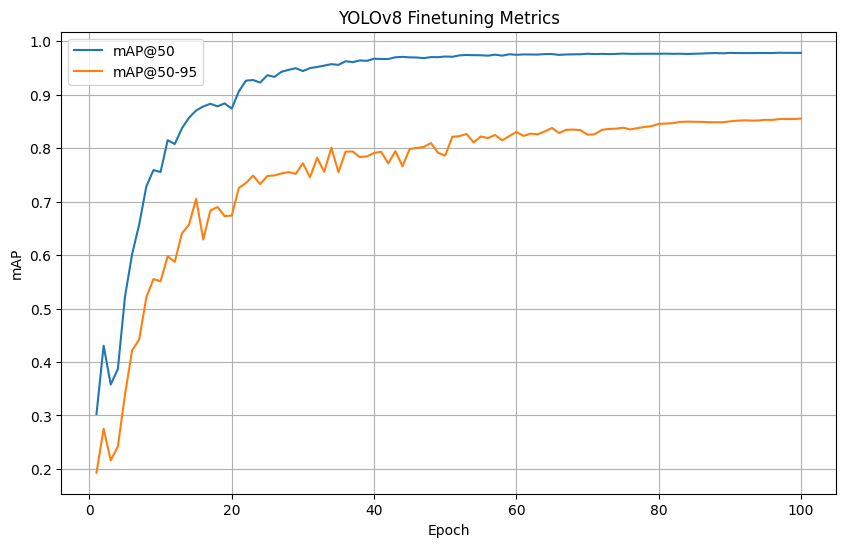
\includegraphics[width=0.8\linewidth]{imgs/detect_finetune_results_val.png}
    \caption{Mean Average Precision at threshold confidence 0.5 and 0.5-0.95 during fine-tuning}
    \label{fig:det-finetune-mAP}
\end{figure}

\begin{table}[H]
\centering
\begin{tabular}{lcccc}
\toprule
\textbf{Class} & \textbf{Precision} & \textbf{Recall} &
\textbf{mAP\textsubscript{50}} & \textbf{mAP\textsubscript{50--95}} \\
\midrule
Bowl           & 0.996 & 0.904 & 0.905 & 0.817 \\
CanOfCocaCola  & 0.978 & 0.999 & 0.995 & 0.879 \\
FryingPan      & 0.983 & 0.994 & 0.995 & 0.913 \\
Glass          & 0.999 & 0.990 & 0.995 & 0.869 \\
Jam            & 0.975 & 0.890 & 0.984 & 0.873 \\
Lid            & 0.998 & 0.999 & 0.995 & 0.912 \\
MilkBottle     & 0.999 & 0.983 & 0.995 & 0.888 \\
Mug            & 0.990 & 0.995 & 0.995 & 0.898 \\
OilBottle      & 0.978 & 0.999 & 0.994 & 0.874 \\
Plate          & 0.988 & 0.994 & 0.995 & 0.938 \\
Rice           & 0.997 & 0.999 & 0.995 & 0.908 \\
Saucepan       & 0.982 & 0.967 & 0.983 & 0.883 \\
Sponge         & 0.994 & 0.973 & 0.975 & 0.847 \\
Sugar          & 0.991 & 0.972 & 0.994 & 0.895 \\
VinegarBottle  & 0.982 & 0.984 & 0.994 & 0.869 \\
WashLiquid     & 0.991 & 0.957 & 0.988 & 0.831 \\
\midrule
All (mean)     & 0.989 & 0.975 & 0.986 & 0.881 \\
\bottomrule
\end{tabular}
\caption{Per-class detection results on the test set (fine-tuned \texttt{YOLOv8n})}
\label{tab:det-finetune-results}
\end{table}

Overall, the finetuning yielded extremely good results, achieved high Average Precision for all classes and is suitable for deployment.

\subsection{Detection Samples}
\label{sec:det-samples}

Figures~\ref{fig:det-sample-testset} and \ref{fig:det-sample-ondevice} show representative
detections from the fine-tuned model running the test set and on-device. For on-device sample, bounding boxes are rendered in the passthrough feed at the depth returned by the
environment raycast. The label text shows the detected class and normalized center coordinates.

\begin{figure}[H]
    \centering
    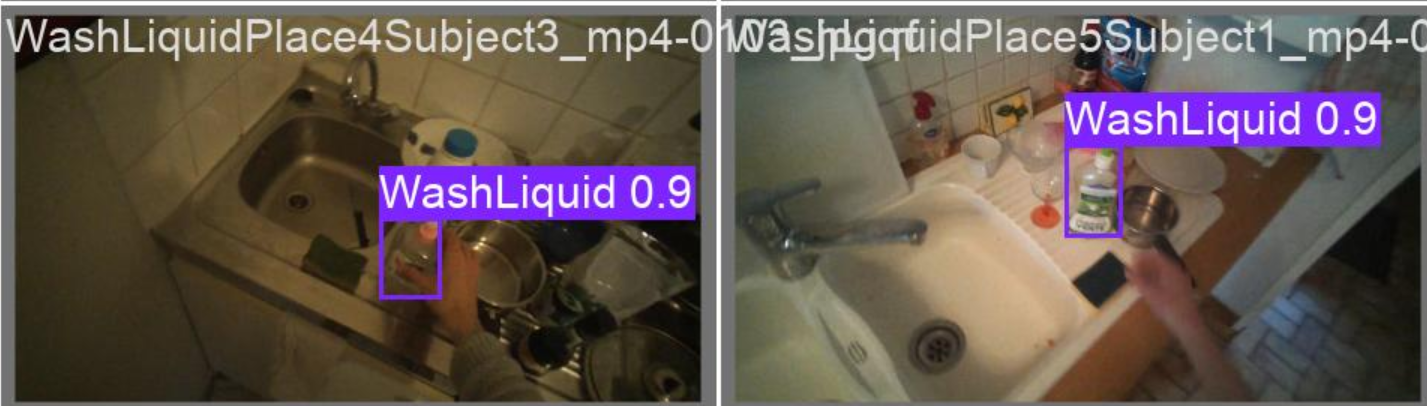
\includegraphics[width=\textwidth]{imgs/detection_model_sample1.png}%
    \vspace{1pt}
    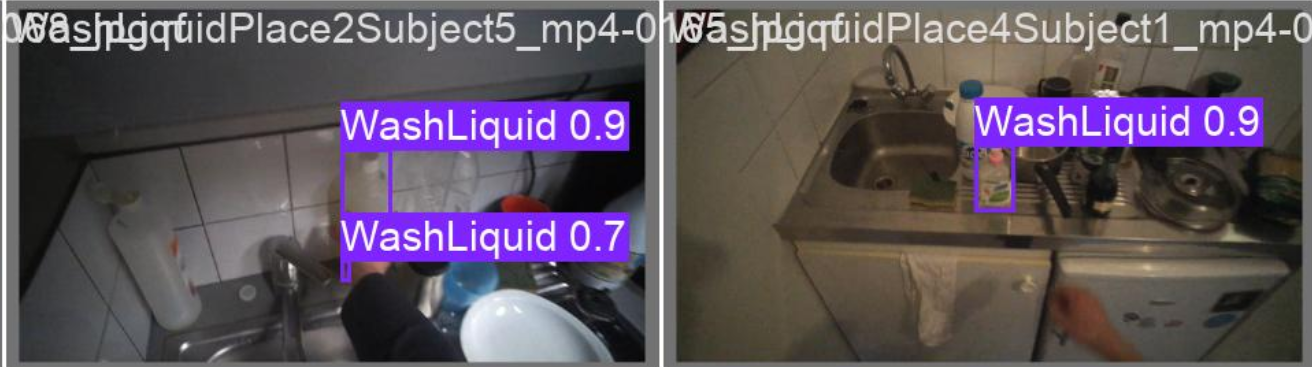
\includegraphics[width=\textwidth]{imgs/detection_model_sample2.png}
    \caption{Detection output running on the test set.}
    \label{fig:det-sample-testset}
\end{figure}
    
\begin{figure}[H]
    \centering
    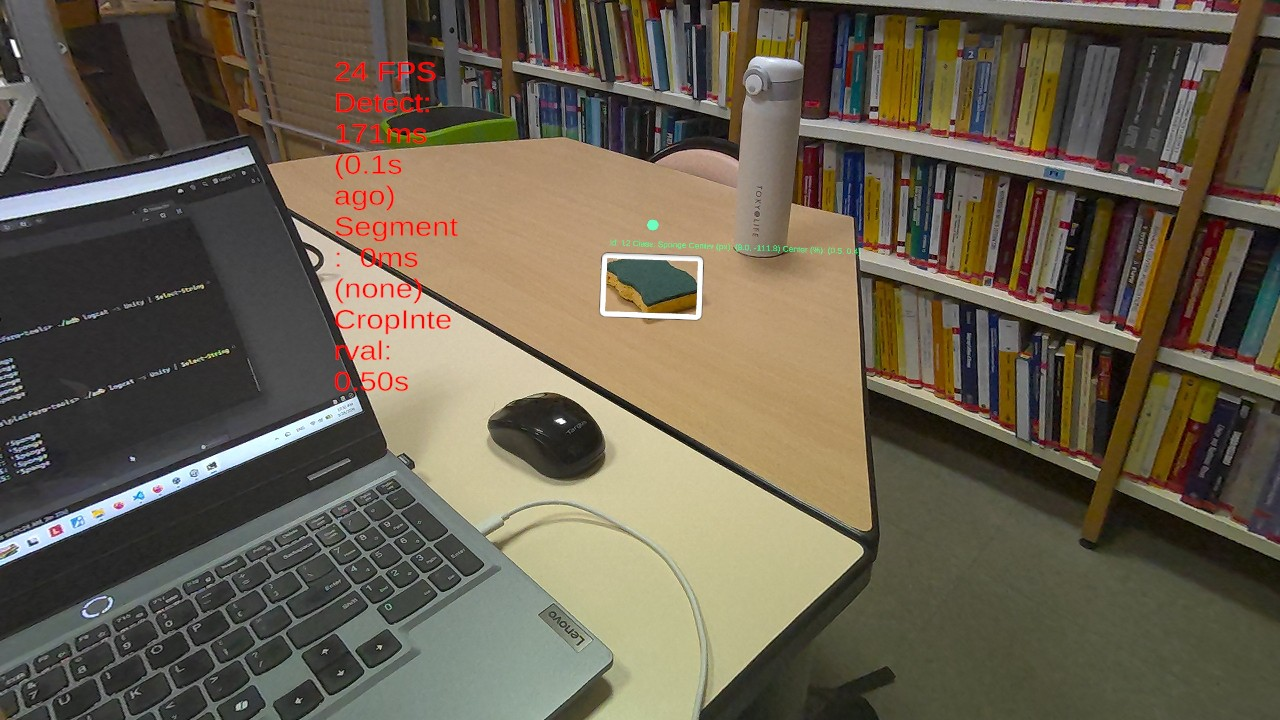
\includegraphics[width=\textwidth]{imgs/detection_roi_sample1.jpg}
    \caption{Detection output running on-device, green dot shows direction of the headset which is used in the next section. (Note: due to the FOV of the Meta Quest, the image looks much wider compared to what we see on-device)}
    \label{fig:det-sample-ondevice}
\end{figure}

% \newpage
\section{Head gaze}

\subsection{Overview}
The head gaze (the forward direction vector of the headset) serves as a tolerant, hands-free method to select a detected object before cropping its region of interest and passing it to the segmentation model. Rather than requiring precise pointing, the system continuously evaluates which bounding box the user is most directly looking at, providing low-fatigue interaction suited for extended use.

\subsection{Method}
% (Detailed explanation of the method displayed in the graph)

The methodology is illustrated in the following diagram:
\begin{figure}[H]
\centering
\begin{tikzpicture}[
    >=Stealth, 
    every node/.style={draw, rectangle, rounded corners, minimum width=2cm, 
                       minimum height=1cm, align=center},
    image node/.style={inner sep=0pt, draw=none} 
]
    \node[image node] (A) at (0,0) {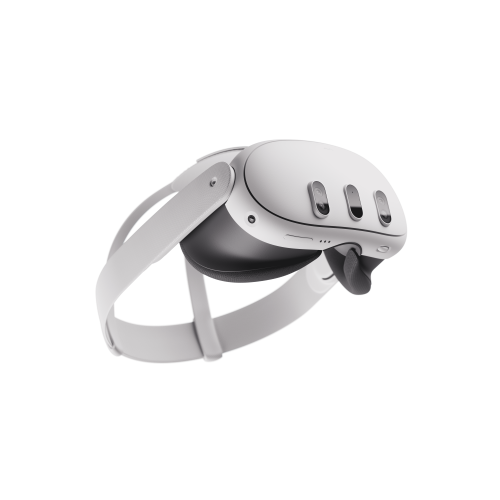
\includegraphics[width=2cm]{imgs/mq3.png}}; 
    \coordinate (CenterRight) at (4,0);
    \node (B) at (4, 2) {Direction of head gaze};
    \node (C) at (4, 0) {Bounding box's center};
    \draw[->, thick] (A.center) -- (B.west) coordinate[pos=0.6] (arrow1);
    \draw[->, thick] (A.center) -- (C.west) coordinate[pos=0.6] (arrow2);
    \path pic [draw, <->, "$\theta$", angle radius=1.5cm, angle eccentricity=1.2, 
               nodes={draw=none}] {angle = C--A--B};
    \draw[<->, thick] (B.south) -- (C.north) 
        node[midway, right, draw=none] 
            {Hit Distance = $\frac{\text{Box diagonal}}{2}$};
\end{tikzpicture}
\caption{Selecting a region of interest via head gaze.}
\label{fig:headgaze}
\end{figure}


At each frame, the headset's forward axis defines a \textit{gaze ray} originating from the center eye anchor. Every bounding box in world space exposes a center point and a world-space size. The selection proceeds in three steps:

\begin{itemize}
    \item \textbf{Ray-to-box proximity test.} The perpendicular distance from each 
    bounding box's world-space center to the gaze ray is compared against a hit radius 
    equal to half the box's world-space diagonal. Boxes within this radius become 
    candidates.

    \item \textbf{Best-candidate selection.} Among all candidates, the box subtending 
    the smallest angle $\theta$ with the gaze direction is selected 
    , i.e.\ the one most centrally aligned with the line 
    of sight.

    \item \textbf{Selection persistence.} The current selection is held until a 
    different box strictly wins the angle comparison, suppressing flicker between 
    adjacent boxes without an explicit debounce timer.
\end{itemize}
Once a box is selected, its normalised image-space coordinates are forwarded to the cropping stage.

\subsection{Demonstration}

\begin{figure}[H]
    \centering
    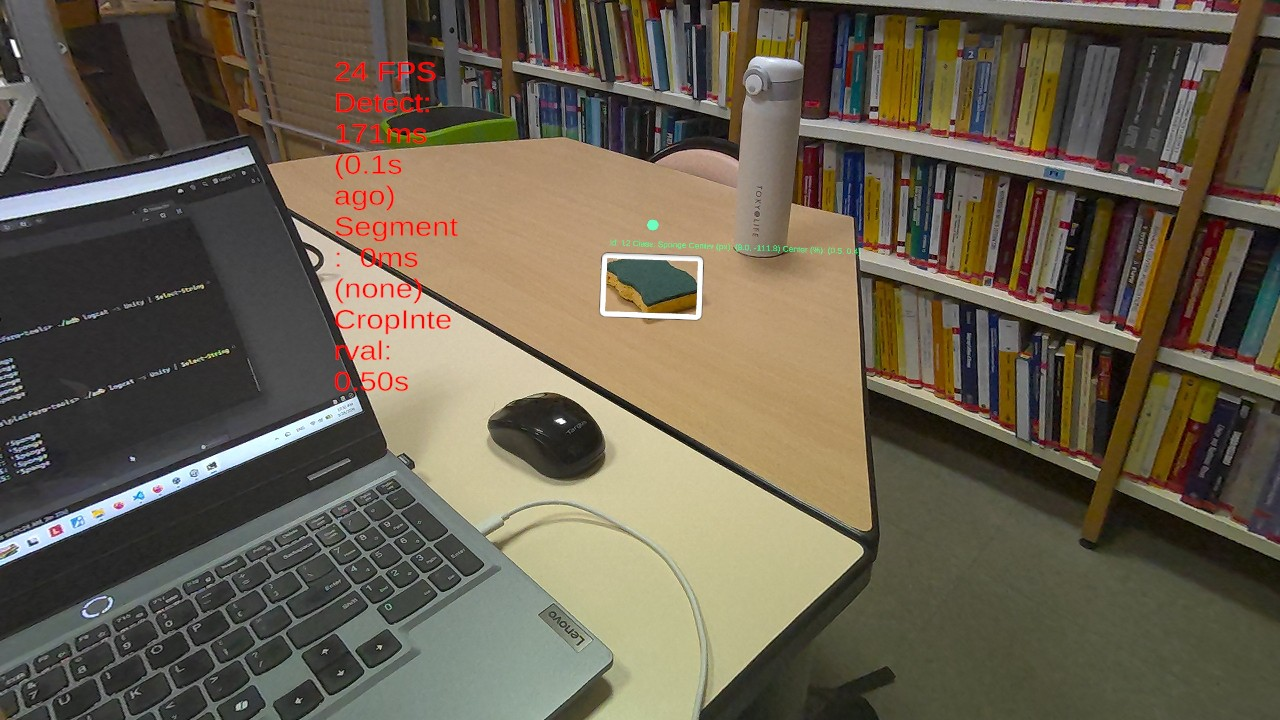
\includegraphics[width=\linewidth]{imgs/detection_roi_sample1.jpg}
    \caption{Before selection, gaze indicated by a green dot}
    \label{fig:before}
    
    \vspace{1em} 
    
    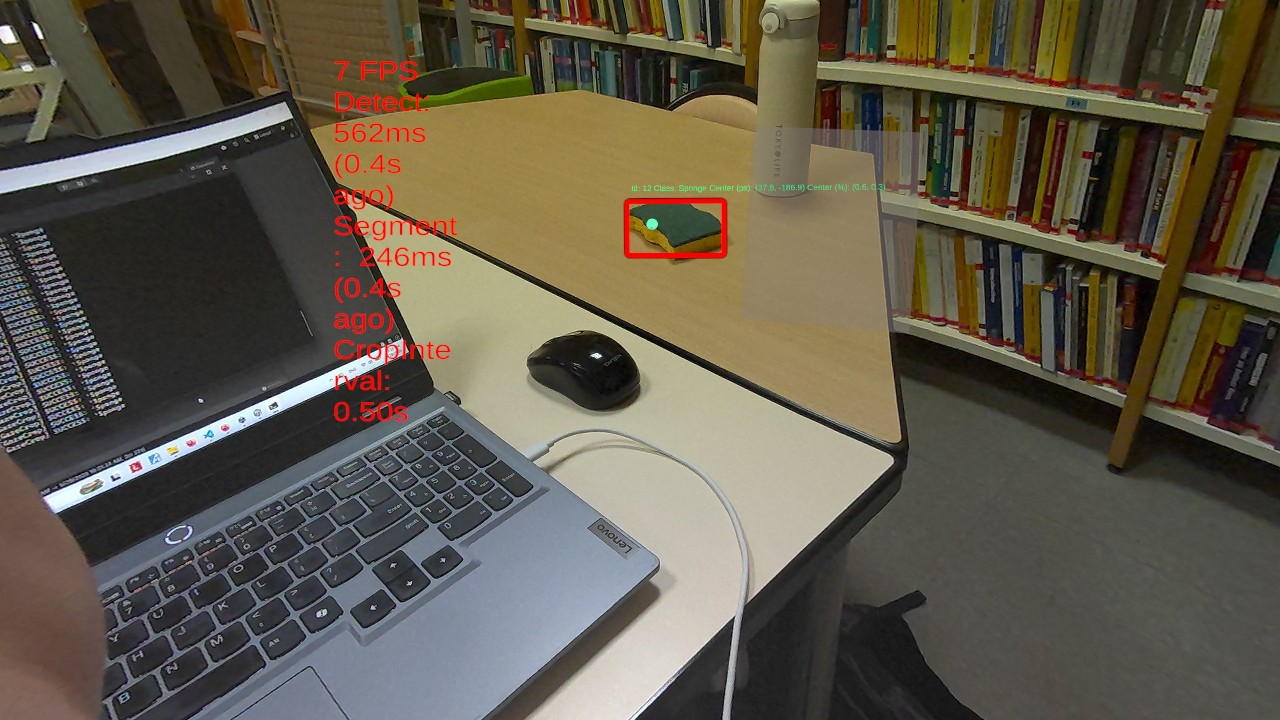
\includegraphics[width=\linewidth]{imgs/detection_roi_sample2.jpg}
    \caption{After selection, gaze indicated by a green dot, and a panel on the right showing custom json description.}
    \label{fig:after}

\end{figure}

\newpage
\section{Cropping ROI}

\subsection{Overview}
Once a bounding box is selected via head gaze, its region of interest (ROI) is extracted
from the camera frame and forwarded to the segmentation model. The crop is expanded by a
fixed margin of 10\% on each side to ensure the object's boundary is fully enclosed,
compensating for slight misalignments between the detection box and the true object
extent.

\subsection{Converting Pixel Data Between Spaces}
The bounding box produced by the detection model is stored as normalised coordinates in
$[0, 1]^2$ relative to the $640 \times 640$ input tensor. To crop the correct region
from the raw camera frame, these coordinates are mapped to camera pixel space in two
steps :

\begin{itemize}
    \item \textbf{Model space $\to$ camera pixel space.} The normalized box coordinates
    are multiplied by the camera's native resolution to obtain pixel-space
    coordinates. 

    \item \textbf{Margin expansion.} The box is expanded by 10\% of its width and height
    on all four sides before cropping, then resized down or letterbox-padded to 640x640.
\end{itemize}

The crop is then blitted (blit - copy pixel data to another buffer) into a smaller \texttt{RenderTexture} entirely on the GPU using
a scaled \texttt{Graphics.Blit} call, avoiding any CPU readback of the full-resolution
frame. The resulting texture is forwarded to the segmentation pipeline.

\subsection{Limitations}
\begin{itemize}
    \textbf{Latency:} The ROI is extracted at a fixed interval (default 100\,ms) to reduce the number of images sent for segmentation. The segmentation therefore runs on a crop that may be slightly old relative to the current passthrough view. Fast-moving objects or sudden head rotation between extraction and display may cause mask misalignment.

    % \item \textbf{Resolution loss:} Cropping a small or distant object from the
    % full-resolution frame and resizing it to $640 \times 640$ for the segmentation model
    % can degrade mask quality. 
\end{itemize}

\subsection{Samples}
\begin{figure}
    \centering
    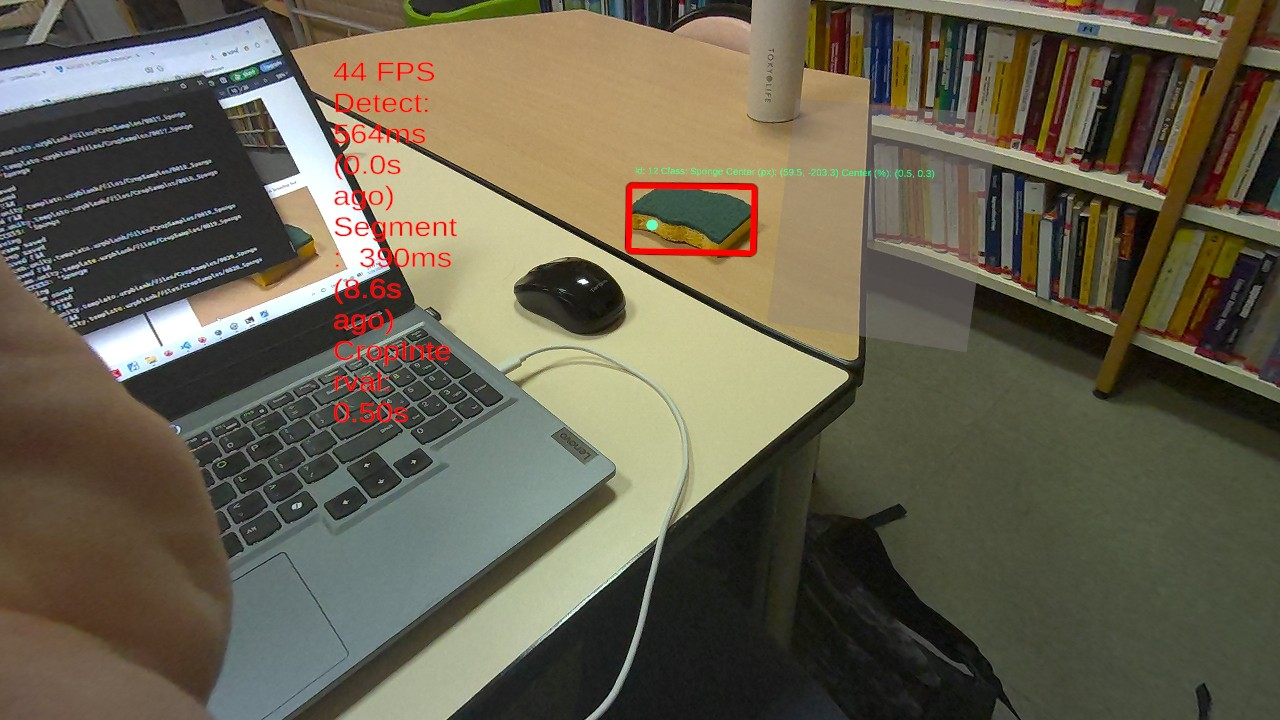
\includegraphics[width=\textwidth]{imgs/detection_crop_roi_sample1.jpg}
    \caption{Frame with a selected object, its detection bounding box and a panel on the right showing custom json drescription.}
    \label{fig:detection-roi}

    \vspace{1em} 

    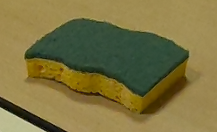
\includegraphics[width=0.7\textwidth]{imgs/detection_crop_roi_sample2.png}
    \caption{The extracted crop forwarded to the semantic segmentation model.}
    \label{fig:cropped-roi}
\end{figure}

\newpage
\section{Semantic Segmentation}

\subsection{Overview}
Once a region of interest (ROI) has been extracted from the camera frame, it is forwarded to an semantic segmentation model that
produces a per-pixel binary mask identifying the selected object. The mask is then
projected back into world space and displayed as a semi-transparent overlay on the
passthrough feed, co-planar with the detected box surface at the depth returned by the
environment raycast.\\

The overlay is positioned by casting rays from the camera through the four corners of
the crop viewport, intersecting them with a plane perpendicular to the gaze direction at
the raycasted depth, and fitting the mask quad to the resulting world-space rectangle.
Transparent pixels in the mask texture naturally clip the visible region, so no
additional geometry is required.

% ─────────────────────────────────────────────────────────────────────────────
\subsection{Model Choice}

Selecting a segmentation model for the Meta Quest~3 requires balancing mask quality
against hard latency constraints, with inference running asynchronously alongside
the detection pipeline.

\paragraph{YOLO26n-sem.}
YOLO26~ is Ultralytics' \cite{ultralytics_yolo26} latest edge-first model family, released in
January~2026. The nano segmentation variant, \texttt{yolo26n-sem}, released in May 20th, pretrained on the \textbf{Cityscapes} dataset, weighs only 3.3\,MB
and introduces several architectural improvements relevant to this application:

\begin{itemize}
    \item \textbf{MuSGD Optimizer for Stable Convergence:} MuSGD leverages the robustness and generalization capacity
    of SGD while incorporating adaptive properties from Muon, enabling faster convergence and more stable optimization across diverse datasets.
    
    \item \textbf{Upgraded proto module.} A multi-scale prototype module improves mask quality for objects of varying size and in complex scenes.
\end{itemize}

\noindent Given the latency and memory constraints, \texttt{yolo26n-sem} was selected
and fine-tuned on the Grasping-In-The-Wild dataset.\\

Other architecture were considered, including Meta's Segment Anything Model~2 (SAM~2) and its distilled derivatives
MobileSAM and TinySAM, which were used in some researches of the IWRIST project. Unfortunately, none of them produces a performance above the 3.7\,FPS required for real-time operation, so the idea was quickly dismissed.

\subsection{Fine-Tuning}
The COCO-pretrained \texttt{yolo26n-sem} weights were fine-tuned on Grapsing-In-The-Wild dataset to improve mask quality for the target object categories. This section describes the
dataset split, training configuration, and evaluation results.\\

\paragraph{Dataset:}
The dataset was split as follows:

\begin{table}[H]
\centering
\caption{Dataset split used for fine-tuning.}
\label{tab:dataset-split}
\begin{tabular}{lrr}
\toprule
\textbf{Split} & \textbf{Images} & \textbf{Proportion} \\
\midrule
Train      & 9188 & 70\% \\
Validation & 1969 & 15\% \\
Test       & 1969 & 15\% \\
\bottomrule
\end{tabular}
\end{table}

\paragraph{Training configuration.}
Fine-tuning was performed using the Ultralytics training framework with the following
hyperparameters:

\begin{table}[H]
\centering
\caption{Fine-tuning hyperparameters.}
\label{tab:finetune-config}
\begin{tabular}{ll}
\toprule
\textbf{Parameter} & \textbf{Value} \\
\midrule
Base weights     & \texttt{yolo26n-sem.pt} \\
Input resolution & $640 \times 640$ \\
Epochs           & 100 \\
Batch size       & 32 (16 per GPU) \\
Optimiser        & Auto (Default: SGD) \\
Learning rate    & $0.01$ (Initial $\text{lr}_0$) \\
\midrule
\multicolumn{2}{l}{\textit{Data augmentation}} \\
Mosaic           & On ($1.0$ probability) \\
Random flip      & Left-right ($0.5$ prob.) \\
Colour jitter    & H: $0.015$, S: $0.7$, V: $0.4$ \\
Scale jitter     & $\pm 0.5$ (Gain), Rotation: $\pm 15^\circ$ \\
Copy-paste       & $0.3$ probability \\
\bottomrule
\end{tabular}
\end{table}

\paragraph{Results.}
The fine-tuned model was evaluated on the held-out test set. Training and validation
curves are shown in Figure~\ref{fig:finetune-curves}; per-class metrics are reported
in Table~\ref{tab:finetune-results}.

\begin{figure}[H]
    \centering
    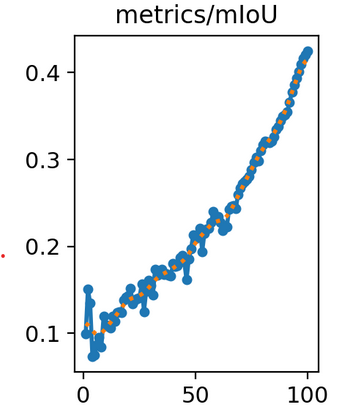
\includegraphics[width=0.4\linewidth]{imgs/sem_training_iou.png}
    \caption{Mean Intersection over Union (mIoU) on the validation set during training over 100 epochs}
    \label{fig:finetune-curves}

    \vspace{1cm}
    
    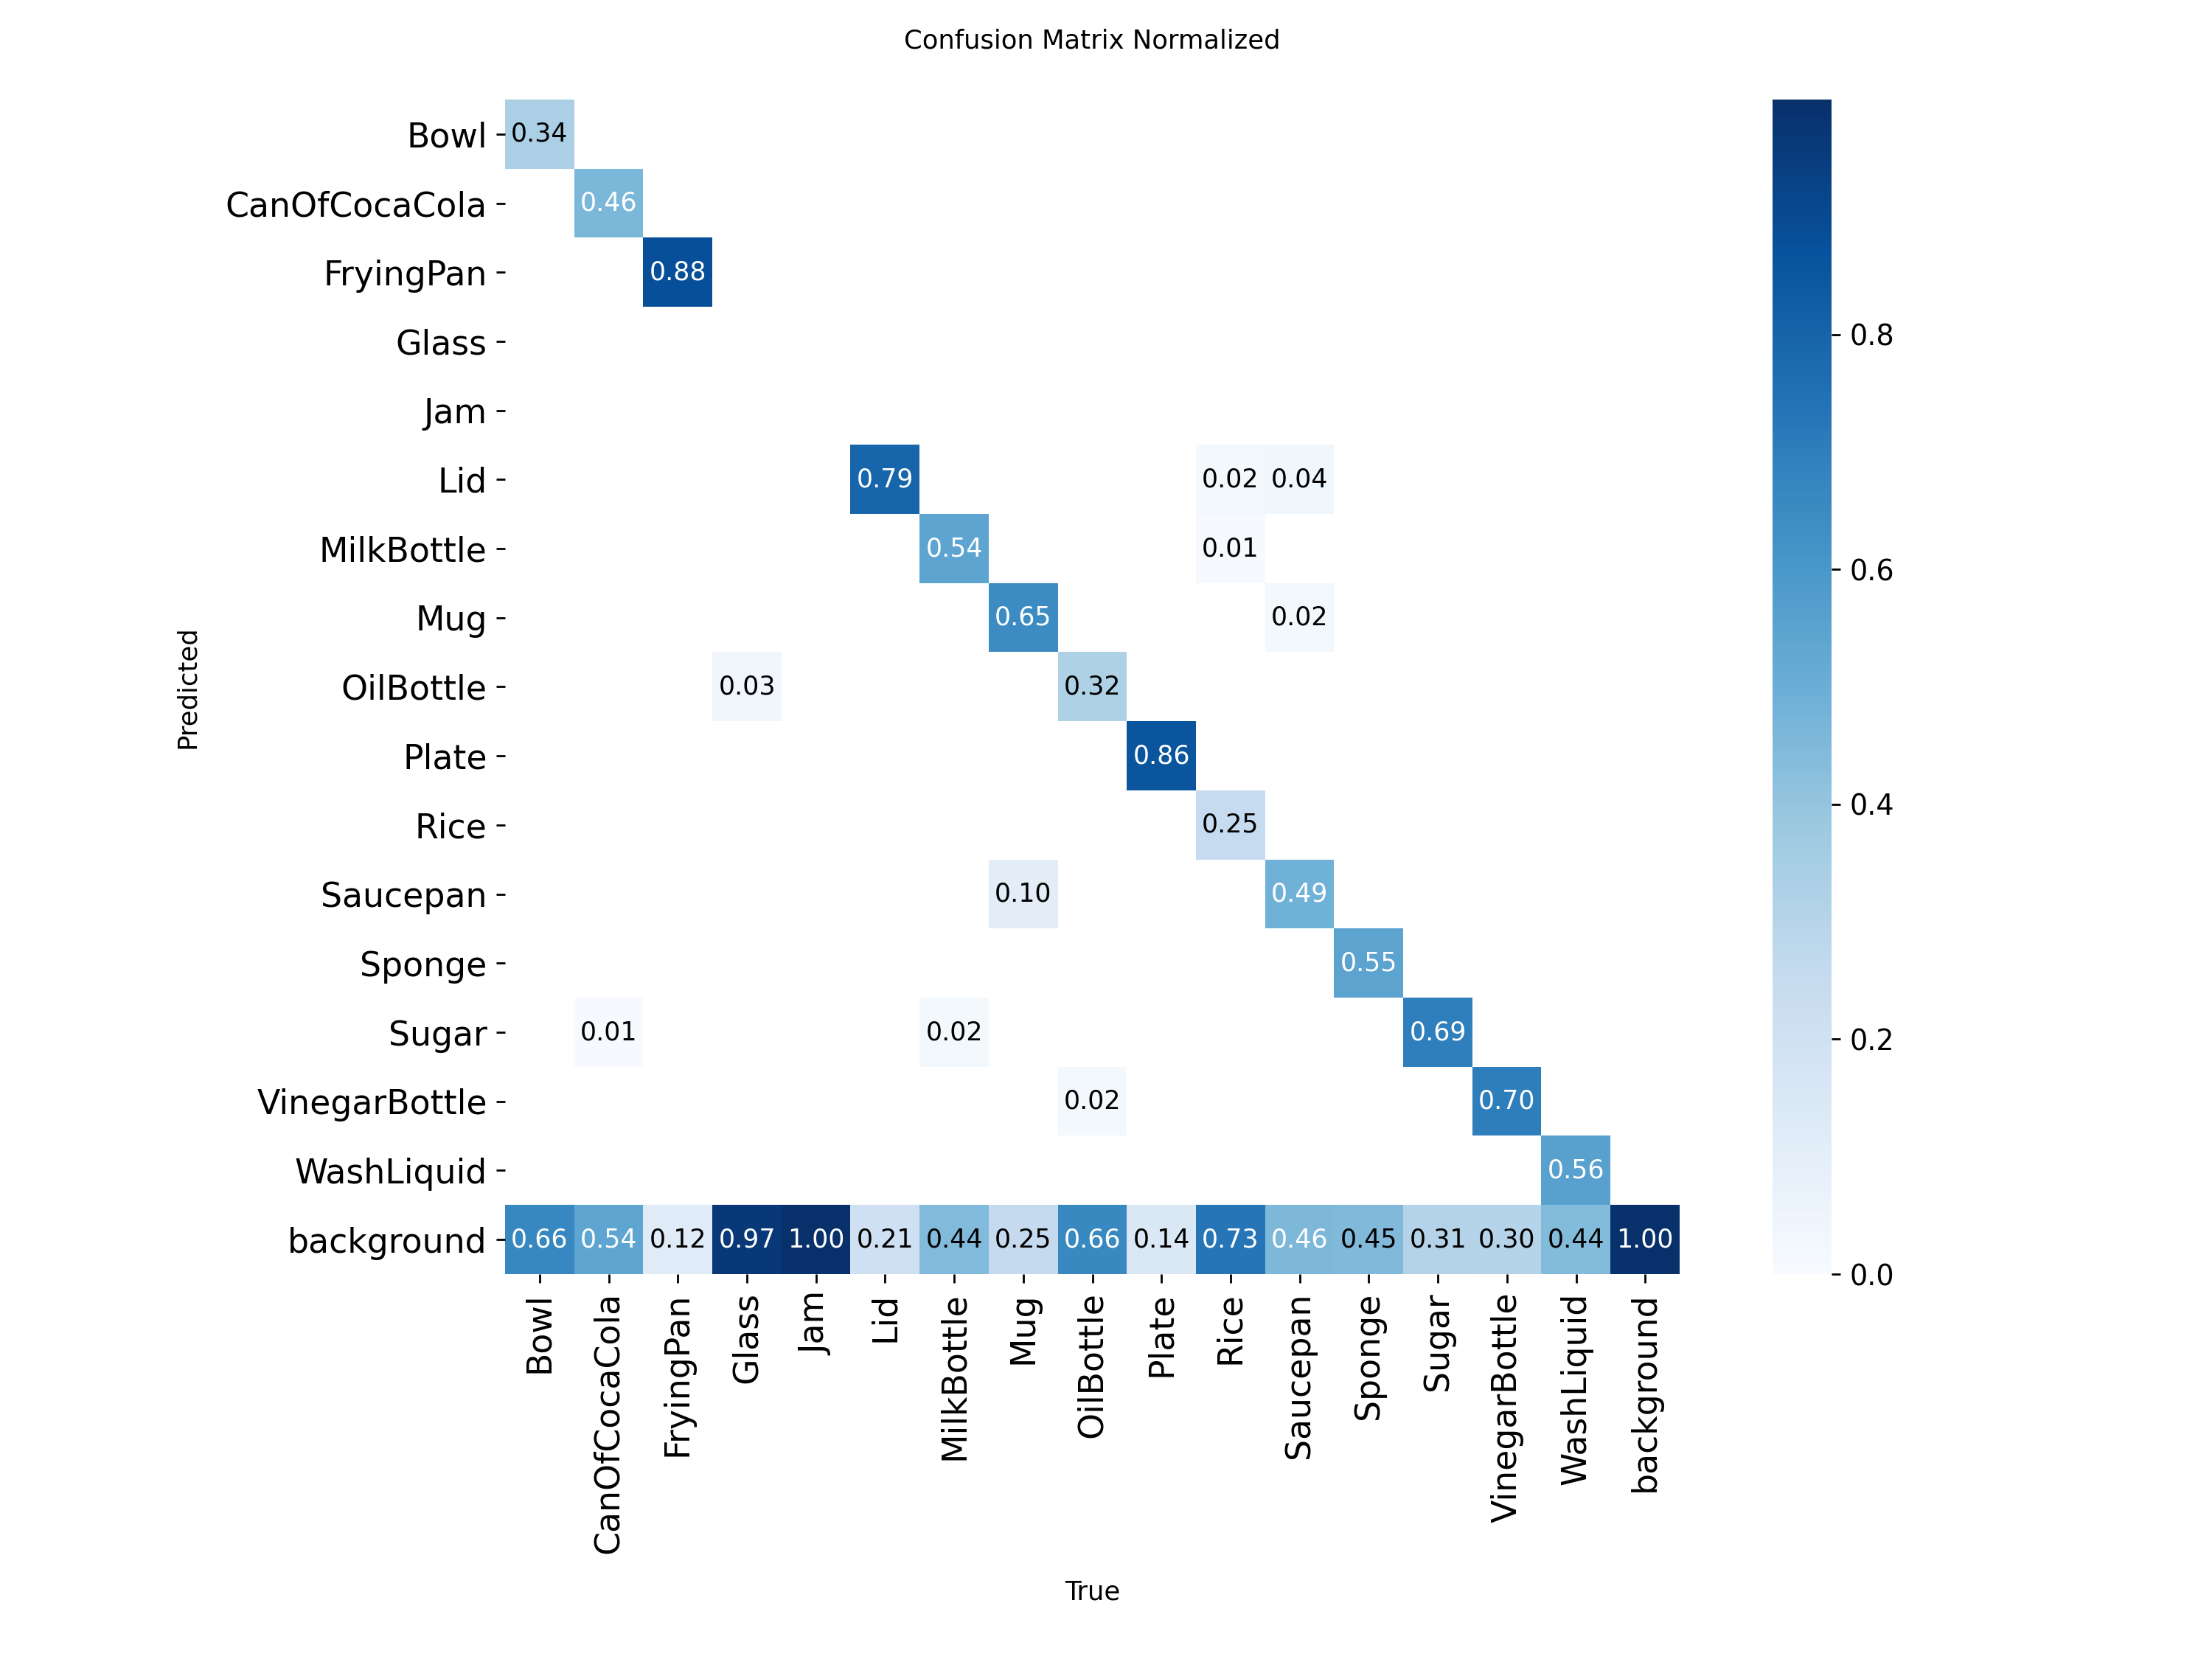
\includegraphics[width=\linewidth]{imgs/segmentation_confmat_norm.png}
    \caption{Normalized Confusion matrix on the test set}
    \label{fig:finetune-confmat}
\end{figure}

\begin{table}[H]
\centering
\begin{tabular}{lc}
\toprule
\textbf{Class} & \textbf{IoU} \\
\midrule
Bowl           & 0.438 \\
CanOfCocaCola  & 0.437 \\
FryingPan      & 0.725 \\
Glass          & 0.000 \\
Jam            & 0.000 \\
Lid            & 0.636 \\
MilkBottle     & 0.508 \\
Mug            & 0.486 \\
OilBottle      & 0.235 \\
Plate          & 0.630 \\
Rice           & 0.208 \\
Saucepan       & 0.512 \\
Sponge         & 0.363 \\
Sugar          & 0.456 \\
VinegarBottle  & 0.365 \\
WashLiquid     & 0.000 \\
background     & 0.000 \\
\midrule
All (mean)     & 0.353 \\
\bottomrule
\end{tabular}
\caption{Per-class evaluation of the fine-tuned \texttt{yolo26n-sem} model on the test set.}
\label{tab:finetune-results}
\end{table}

\noindent \textbf{Analysis of Preliminary Results:} As indicated in Table~\ref{tab:finetune-results}, several highly challenging or transparent object classes (e.g., \textit{Glass}, \textit{WashLiquid}) currently display an IoU of $0.000$. 

Still, at the time of reporting, the training is incomplete and the current semantic segmentation model will receive further finetuning until the end of my internship, which is about 3 weeks from now. Because the validation mIoU curve exhibits a steady upward trajectory without plateauing (Figure~\ref{fig:finetune-confmat}), the metrics are expected to rise.

Also, it is important to note that, based on the confusion matrix, most of the wrong predictions are from the cases where the model confuses the object with the background. Meanwhile, there are very few cases where different objects are mistaken for each other.

\subsection{Semantic Segmentation Samples} 


\begin{figure}[H]
    \centering
    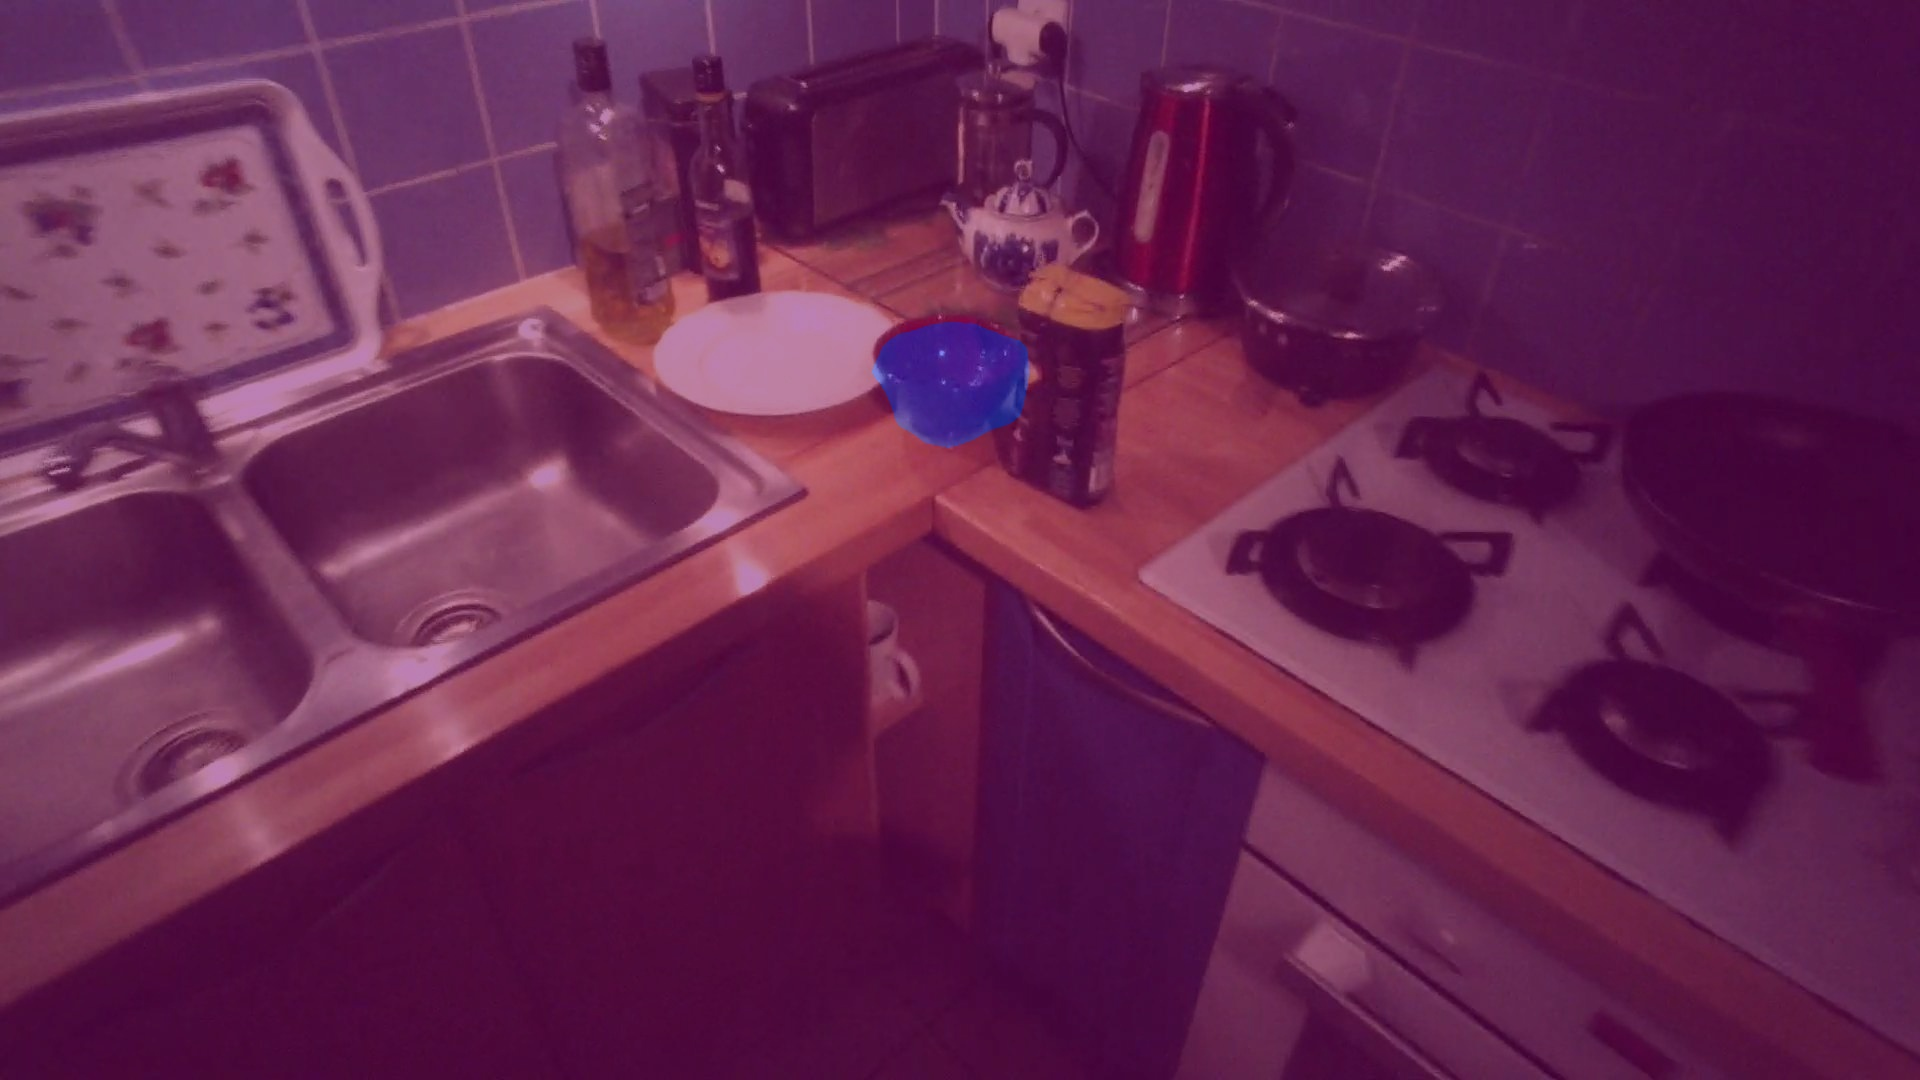
\includegraphics[width=\textwidth]{imgs/segmentation_sample1.jpg}
    \caption{Semantic segmentaion output running on the test set.}
    \label{fig:seg-sample-1}

    \vspace{1em} 

    \centering
    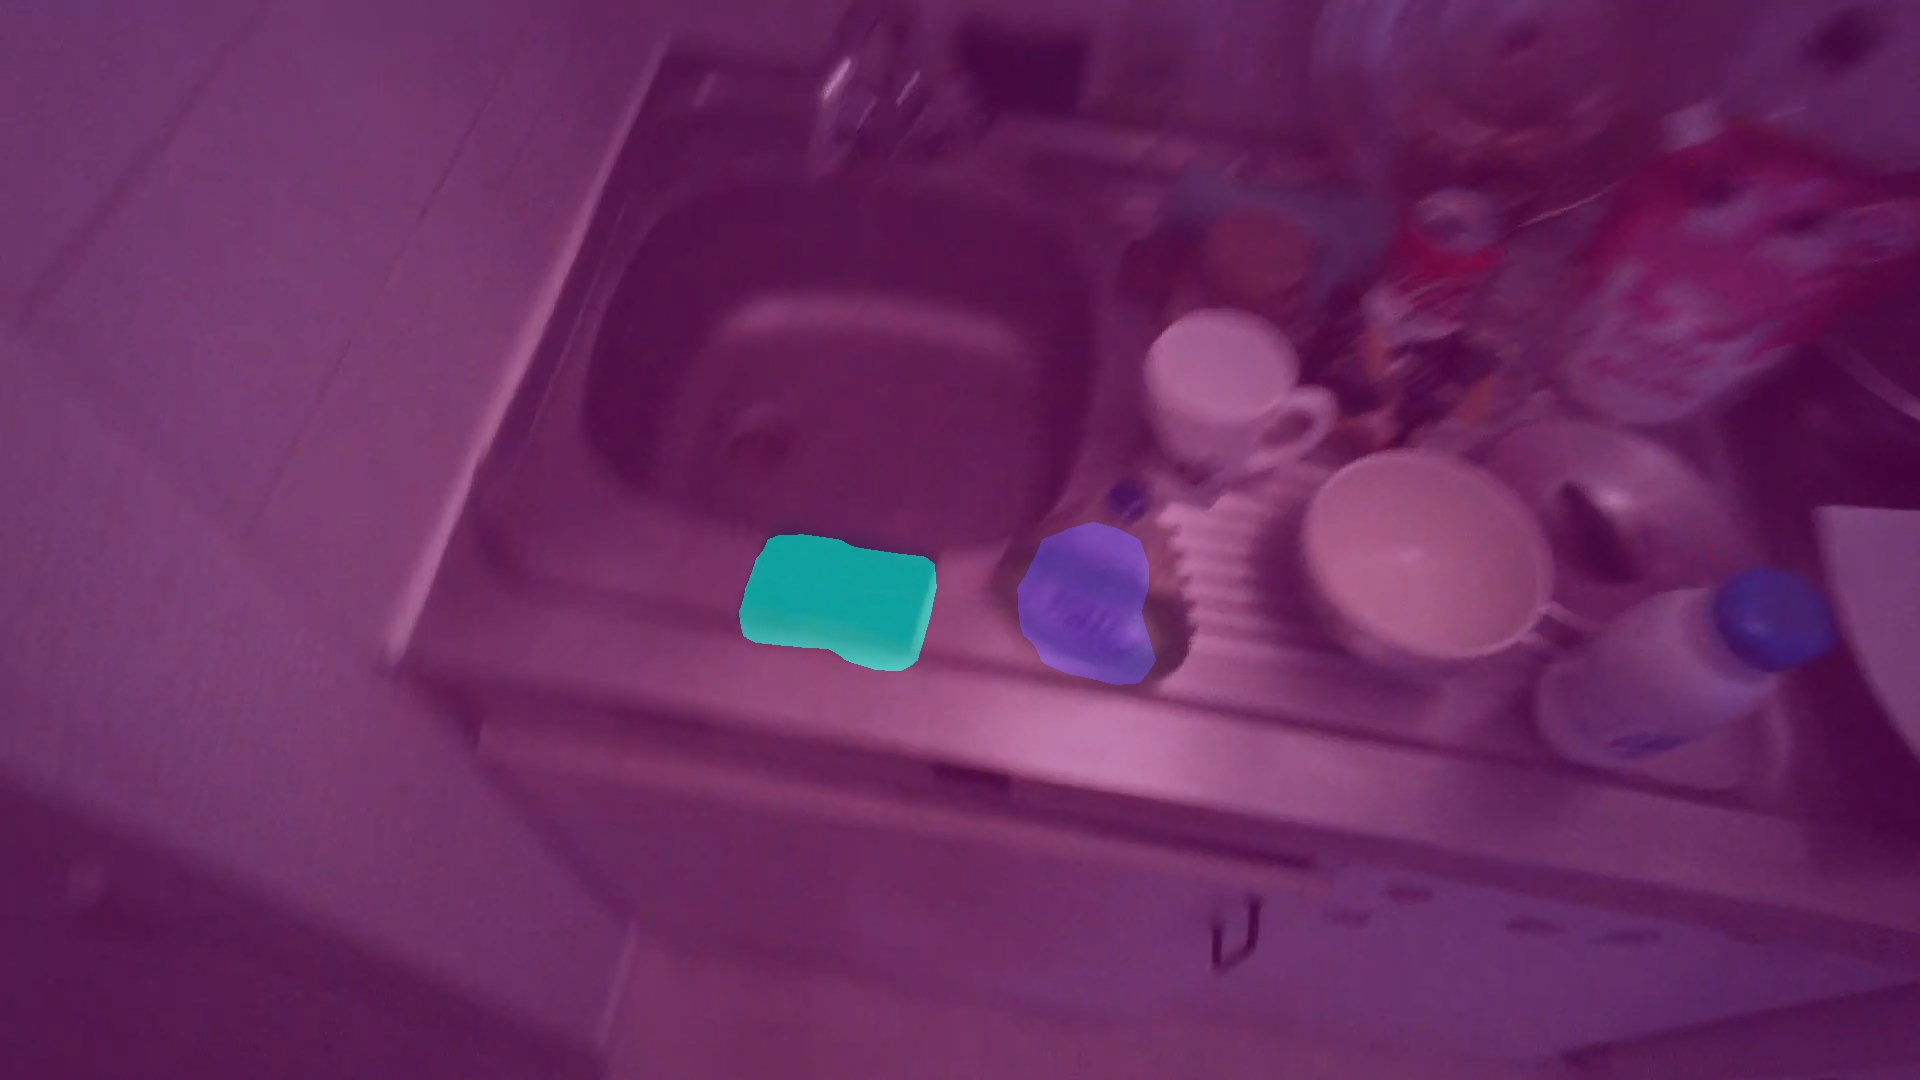
\includegraphics[width=\textwidth]{imgs/segmentation_sample2.jpg}
    \caption{Semantic segmentaion output running on the test set.}
    \label{fig:seg-sample-2}
\end{figure}

\newpage
\section{Possible Improvements}

I propose a few techniques that can improve the quality of my work for the rest of my internship, as well as some ideas for future development.

\subsection{Optimizing graphics rendering}
Meta Quest 3 supports \href{https://developers.meta.com/horizon/documentation/unity/os-fixed-foveated-rendering/}{\textbf{fixed foveated rendering (FFR)}}. FFR enables the edges of an application-generated frame to be rendered at a lower resolution. By using this technique, we can potentially improve framerate and reduce GPU's workload.

\subsection{Reducing Inference Latency}
To lower the inference speed of the processing pipeline, an strategy was proposed to ensure reliability in real-time applications.\\

% (Explanation)\\
Given that the detection stage does not require a precise prediction, we can use a more primitive approach to track the targeted object without having to run the detection frequently.\\

\textbf{Template matching} is a classical computer vision technique where a small reference image (the template) is slid across a larger image to find regions that look similar. We can use this method to track the select object, using the segmented area as a template, and only rerun the detection after the head gaze has moved away from the object or after a short interval.

% (Diagram)\\
\begin{figure}[htbp]
\centering
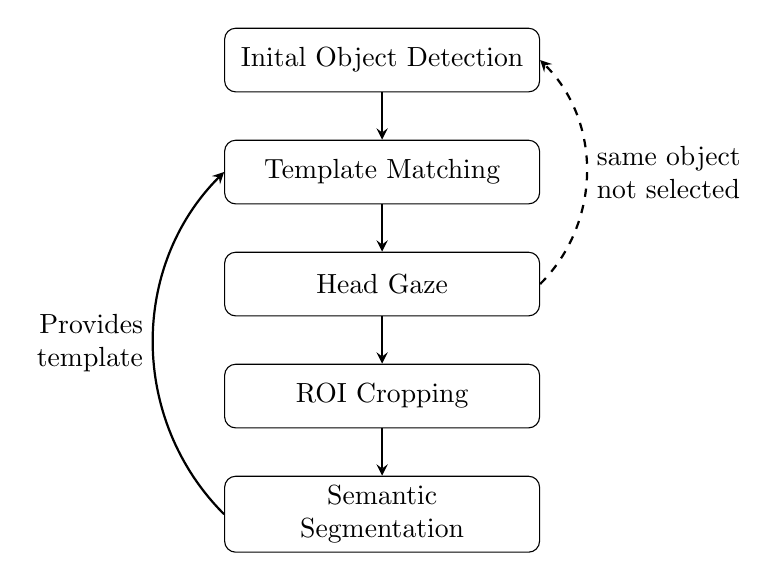
\begin{tikzpicture}[
    % Set a uniform vertical gap of 0.6cm between all blocks
    node distance=0.6cm,
    box/.style={rectangle, draw, rounded corners, align=center, minimum width=4cm, minimum height=2.3em},
    arrow/.style={-stealth, thick}
]
    \node[box] (b1) {Inital Object Detection};
    \node[box] (tm) [below=of b1] {Template Matching};
    \node[box] (b2) [below=of tm] {Head Gaze};
    \node[box] (b3) [below=of b2] {ROI Cropping};
    \node[box] (b4) [below=of b3] {Semantic \\ Segmentation};

    \draw[arrow] (b1) -- (tm);
    \draw[arrow] (tm) -- (b2);
    \draw[arrow] (b2) -- (b3);
    \draw[arrow] (b3) -- (b4);

    \draw[arrow, black] (b4.west) to[bend left=45] 
        node[midway, left, draw=none, text=black, align=right] {Provides \\ template} (tm.west);
        
    \draw[arrow, black, dashed] (b2.east) to[bend right=45] 
        node[midway, right, draw=none, text=black, align=left] {same object \\ not selected} (b1.east);
\end{tikzpicture}
\caption{Overview of the optimized pipeline.}
\label{fig:pipeline-overview}
\end{figure}


\subsection{Integrating the IWRIST's Algorithm to Meta Quest}

% (Overview)\\
The IWRIST team has developed a sophisticated object pose estimation Deep Learning model \cite{etxezarreta2025first} to predict shape, position, and orientation of an object. We can replace the semantic segmentation with this to further complete the pipeline.\\

% (Diagram of full pipeline after integration)\\
\begin{figure}[H]
\centering
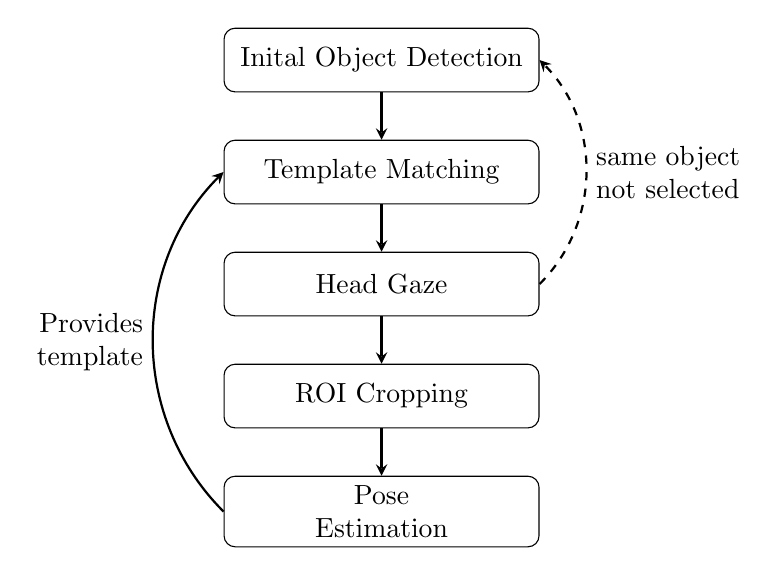
\begin{tikzpicture}[
    % Set a uniform vertical gap of 0.6cm between all blocks
    node distance=0.6cm,
    box/.style={rectangle, draw, rounded corners, align=center, minimum width=4cm, minimum height=2.3em},
    arrow/.style={-stealth, thick}
]
    \node[box] (b1) {Inital Object Detection};
    \node[box] (tm) [below=of b1] {Template Matching};
    \node[box] (b2) [below=of tm] {Head Gaze};
    \node[box] (b3) [below=of b2] {ROI Cropping};
    \node[box] (b4) [below=of b3] {Pose \\ Estimation};

    \draw[arrow] (b1) -- (tm);
    \draw[arrow] (tm) -- (b2);
    \draw[arrow] (b2) -- (b3);
    \draw[arrow] (b3) -- (b4);

    \draw[arrow, black] (b4.west) to[bend left=45] 
        node[midway, left, draw=none, text=black, align=right] {Provides \\ template} (tm.west);
        
    \draw[arrow, black, dashed] (b2.east) to[bend right=45] 
        node[midway, right, draw=none, text=black, align=left] {same object \\ not selected} (b1.east);
\end{tikzpicture}
\caption{Overview of the optimized pipeline.}
\label{fig:pipeline-overview}
\end{figure}

\newpage
\section{Conclusion}

% (Summery of the internship + project)\\
This internship at the MIA laboratory, focusing on developing a detection and semantic segmentation pipeline on the Meta Quest 3 device. \\

% (How the goals have been achieved)\\
This project successfully simplified the IWRIST project's pipeline for initial migration to the Meta Quest device by finetuning a YOLOv8n and a YOLO26n-sem model for a workflow lightweight enough for on-device inference. The performance of the models were assessed using Intersection over Union (IoU) and Average Precision (AP). The resulting pipeline reaches a average frame rate of $\sim$15, suitable for Augmented Reality (AR) experience. \\

However, there are still some issues with the integration of the semantic segmentation model and further training for this model is required. Nevertheless, knowing that the internship period have yet to terminate, these problems will be addressed during the internship. In addition, the remaining duration of the internship would also be used to create a more in-depth, technical documentation of the project, as well as to further optimize the workflow.\\


% (How the project can help the IWRIST's development)\\
This lightweight pipeline can later on serve as a functional proof-of-concept for the IWRIST project's real-time deployment on Meta Quest. It unlocks standalone edge processing, allowing the main project to run complex computing tasks directly on-device with acceptable latency.\\

% (Summery of future plans)\\
Future work will focus on integrating classical computer vision tracking alongside the full-scale IWRIST models. To maximize frame rates, a template matching strategy will bypass frequent object detection by utilizing the segmented region as a template. Ultimately, the semantic segmentation module will be swapped for IWRIST's full 6D object pose estimation model to deliver complete shape, position, and orientation tracking.

\newpage
\bibliographystyle{plainurl}
\bibliography{index}

\end{document}